% legecy/pf/vfh
\بخش{الگوریتم‌های اولیه}
همان‌طور که در ابتدای این فصل آمده است، روش‌های \جام حالت کلی به دو دسته‌ی طرح‌ریزی سراسری و حسگر-مبنا تقسیم می‌شوند و همانطور که قبلا نیز آورده شده است به دلیل عدم کاربری روش‌های طرح‌ریزی سراسری در ربات هدف این پژوهش از ارائه و پیگیری این نوع از روش‌ها در این تحقیق اجتناب می‌کنیم. در مورد الگوریتم‌های اولیه\زیرنویس{\مق{Legacy Algorithms}} که موفق عمل کرده‌اند می‌توان به الگوریتم‌های میدان پتانسیل(\مق{PF}\زیرنویس{\مق{Potential Field}})، میدان نیروی مجازی(\مق{VFF}\زیرنویس{\مق{Virtual Force Field}})، هیستوگرام میدان برداری و بهبودیافته‌اش(\مق{VFH}\زیرنویس{\مق{Vector Field Histogram}} و \مق{VFH+}\زیرنویس{\مق{Vector Field Histogram+}}) اشاره کرد.\بند
در الگوریتم \مق{PF}\مرجع{khatib1986real} که به منظور هدایت بازوهای ربات به سمت موقعیت هدف با محدود عدم برخورد با موانع مشخص موجود در مسیر ارائه شد که بعدها در زمینه‌های دیگر رباتیک بجهت \جام مورد استفاده واقع گردید. در طراحی این روش ربات، موانع محیط و موقعیت هدف به صورت یک نقطه فرض شده است که هریک از این نقاط به صورت مجازی دارای یک بار علامت‌دار می‌باشد که در نتیجه میدان پتانسیلی به جهت جذب و دفع یک دیگر دارند. جنس بارهای ربات و موانع یکسان و مخالف بار موقعیت هدف در نظر گرفته می‌شوند. ربات باتوجه به این اینکه بار آن هم‌علامت موانع بوده به صورت طبیعی از موانع گریزان می‌شود و به سمت هدف جذب می‌گردد؛ مجموع کنش-واکنش ربات/موانع/هدف باعث می‌شود که موانع نیروی دافعه و هدف نیروی جاذبه به ربات اعمال می‌کنند و مسیر حرکت ربات را برآیند این دو نیرو تعیین می‌کند. این روش در کنار سادگی پیاده‌سازی معایب عمده‌ای نیز دارد، اول اینکه باید محیط کاملا شناخته شده باشد دوم اینکه در شرایطی ربات تحت این الگوریتم فلج شده و امکان ادامه‌ی مسیر حتی با وجود مسیر بدون مانع برای ربات مهیا نمی‌شود و این زمانی رخ می‌دهد که مجموع نیرو‌های دافعه و جاذبه روی ربات برابر باشند. به خاطر این معایب این روش کاربردی در رباتیک مدرن نداشته و بیشتر جنبه صنعتی دارد.\بند
الگوریتم \مق{VFF}\مرجع{borenstein1989real} که چند سال بعد از الگوریتم \مق{PF} در \سال{1989} برپایه‌ی ایده‌ای که قبلا الگوریتم میدان پتانسیل ارائه داده بود را برای کاربرد در محیط‌های ناشناخته ارائه شد. در این الگوریتم نیز همانند الگوریتم \مق{PF} ربات تحت تاثیر نیروهای جازبه و دافعه‌ی موقعیت‌های هدف و موانع حرکت می‌کند با این تفاوت که این نیروها توسط موقعیت‌های معین و از پیش تعریف شده محاسبه و اعمال نمی‌گردد بلکه با وقتی موانع توسط حسگرهای ربات که دور تا دور ربات را تحت پوشش قرار داده‌اند حس گردیدند، یک نوع نمایشگر هیستوگرامی در ربات از موانع اطراف خود بوجود می‌آید و به ازای بار حس مانع مقداری از سلول‌ها که مرتب با موقعیت حس شده از مانع می‌باشد بروز رسانی می‌شود. این الگوریتم توانسته است که موقعیت نسبتا خوبی از موانع را در هیستوگرام خود در طی زمان بدست بیاورد. بعد از محاسبه‌ای مقادیر هیستوگرام میزان و جهت نیروی دافعه و جازبه‌ای که باید به ربات برای حرکت به سمت هدف وارد شود محاسبه شده و در نهایت اطلاعات حرکتی به کنترل‌کننده‌ی ربات داده می‌شود، تفاوت این روش با شبکه‌ی قطعیت\مرجع{moravec1985high, moravec1988sensor} در نحوه‌ی بروزرسانی این روش می‌باشد که در پیچیدگی زمانی الگوریتم بسیار موثر است، در \مق{VFF} زمانی که موقعیت یک هدف در هیستوگرام ربات بروز رسانی می‌شود که خانه از جدول به بروز شده ولی در حالی که در شبکه‌ی قطعیت که احتمال وجود موانع محاسبه‌ می‌شود با بروز شدن مقدار یک خانه از جدول مقادیر احتمالی خانه‌های مجاور نیز بروز می‌شود که از نظر محاسباتی پیچیدگی بالایی دارد. لازم به ذکر است که الگوریتم \مق{VFF} نیز به سبب اینکه برای راهبری\زیرنویس{Navigation} همانند \مق{PF} از نیروهای دافعه و جازبه موانع و هدف استفاده می‌کند، به صورت پیش‌فرض معایب راهبری الگوریتم \مق{PF} را نیز دارد.\بند
الگوریتم \مق{VFH}\مرجع{borenstein1991vector} که در \سال{1991} توسط طراح الگوریتم \مق{VFF} برای رفع نواقص آن ارائه شد. در این روش نیز همانند روش \مق{VFF} جدول هیستوگرامی(شکل \ref{fig:vfh_1}) از موانع در ربات تشکیل می‌شود با این تفاوت که در هنگام راهبری بجای استفاده‌ بردارنیرو‌های جازبه و دافعه یک هیستوگرام دیگر از روی هیستوگرام قبلی ساخته می‌شود که میزان چگالی وجود موانع در دور تا دور ربات(یعنی ۰ تا ۳۶۰ درجه) را نمایش می‌دهد سپس با استفاده از این هیستوگرام قطبی\زیرنویس{Polar}(شکل \ref{fig:vfh_2}) جهت حرکت مناسب برای ادامه‌ی مسیر و رفع موانع با درنظر گرفتن یک حد آستانه بدست می‌آید.\بند

\begin{figure}
\centering
\subfigure[هیستوگرام چگالی موانع حس شده از محیط]{ 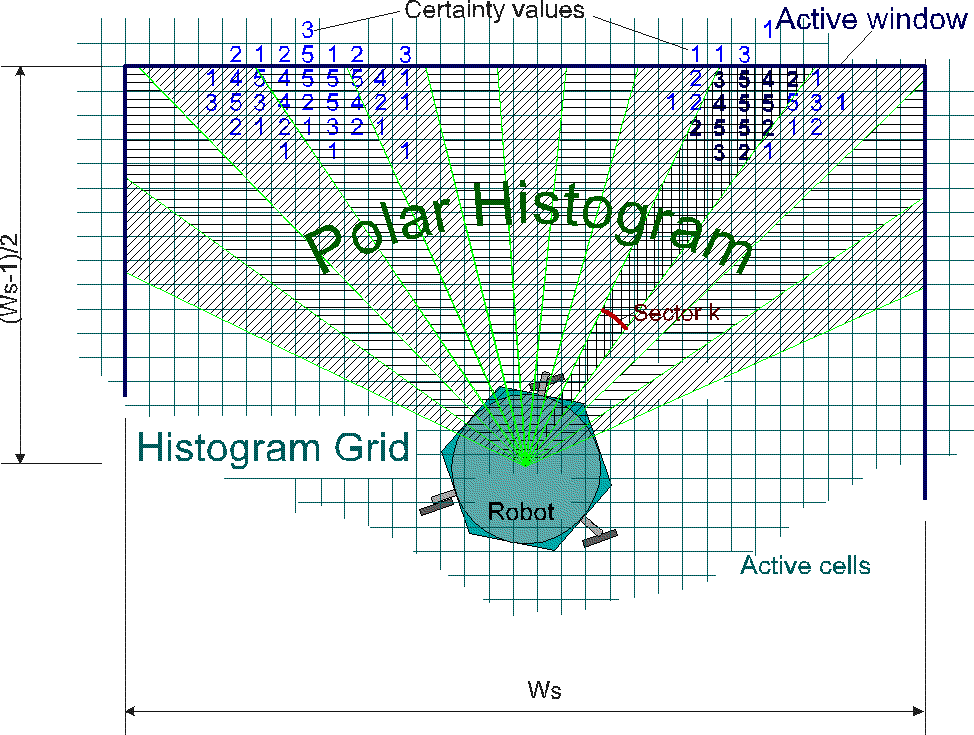
\includegraphics[width=.45\textwidth]{vfh_1}\label{fig:vfh_1} }
\subfigure[هیستوگرام قطبی و حد آستانه بجهت گریز از موانع]{ 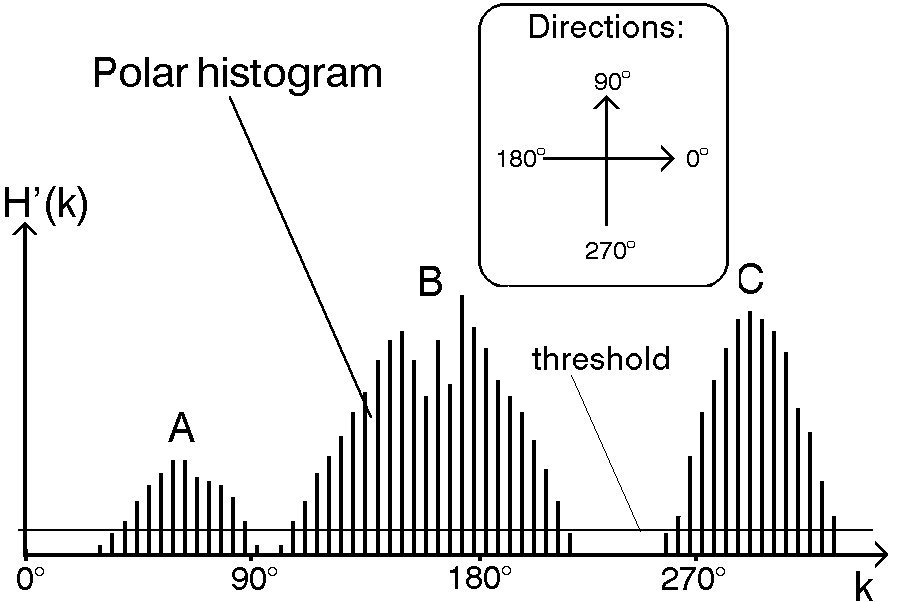
\includegraphics[width=.45\textwidth]{vfh_2}\label{fig:vfh_2} }
\caption{(آ) هیستوگرام‌ چگالی موانع، مورد استفاده در الگوریتم‌های \مق{VFF} و \مق{VFH} - (ب) هیستوگرام قطبی برای راهبری و گریز از موانع، معرفی شده در الگوریتم VFH}
\label{fig:vff_vfh_histo}
\end{figure}

در الگوریتم \مق{VFH+}\مرجع{ulrich1998vfhplus} بهبودیافته الگوریتم \مق{VFH} می‌باشد که در این الگوریتم سعی شده است که احتمال برخورد ربات با موانع کمینه شود. در الگوریتم \مق{VFH} بعد از ساخته شدن هیستوگرام یک مرتبه کاهش بعد داده می‌شود تا به جهت حرکت تعیین شود ولی در الگوریتم \مق{VFH+} این کاهش بعد برای رسیدن به جهت حرکت در ۴ مرحله صورت می‌گیرد؛ به همین دلیل که \مق{VFH+} بعد از گذراندن ۴ مرحله به جهت حرکت دست پیدا می‌کند از نقطه نظر ریاضی اطلاعات کمتری نسبت به \مق{VFH} در طی این فرایند از دست می‌دهد لذا در نهایت ربات را با فرمان‌هایی نرم و مطمئن به حرکت وامی‌دارد.\بند

الگوریتم‌های بالا الگوریتم‌های نسبتا قدیمی هستند ولی به دلیل جامعیت آن‌ها هنوز مقالاتی در رابطه با کاربردها یا بهبودهای مدرن این الگوریتم‌ها ارائه می‌شود. یکی از بهبودهایی که به الگوریتم \مق{PF} در سال‌های اخیر داده شده حل مشکل وقوع قرارگرفتن ربات در کمینه‌ی محلی میدان پتانسیل می‌باشد که الگوریتم \مق{APF\زیرنویس{Adaptive Artificial Potential Field}}\مرجع{rezaee2012adaptive} میدان پتانسیل اطراف موانع را بصورت دورانی تعریف می‌کند و می‌تواند ربات را از قرار گرفتن در کمینه‌های محلی برحذر دارد -- در هنگامی که ربات مستقیما به سمت هدف در حال حرکت است نهایتا به نقطه‌ای خواهد رسید که برایند نیروهای دافعه و جازبه صفر می‌گردد و باعث می‌شود بدون اینکه ربات به مقصد برسد فلج شده و متوقف می‌شود، روش ارائه شده در مقاله مذکور از رخداد این امر جلوگیری می‌کند. \مق{APF} رفتاری سازگار\زیرنویس{Adaptive} با نحوه‌ی همگرایی ربات به مانع دارد. همان طور که در شکل \ref{fig:apf} آمده است زمانی که ربات در میدان پتانسیل مانع قرار می‌گیرد به جهت چرخان بودن این میدان، برآیندی از نیروی چرخشی وارده از سمت میدان و سرعت کنونی ربات جهت‌گیری متناسب با جهت حرکت(معمولا نرم -- مگر در مواقعی که ربات به صورت عمود به سمت مانع حرکت کند) برای اجتناب از برخورد با مانع صورت می‌گیرد.

\begin{figure}
\centering
\subfigure[نمایش عملکرد \مق{APF} از بعد $z-y$]{ 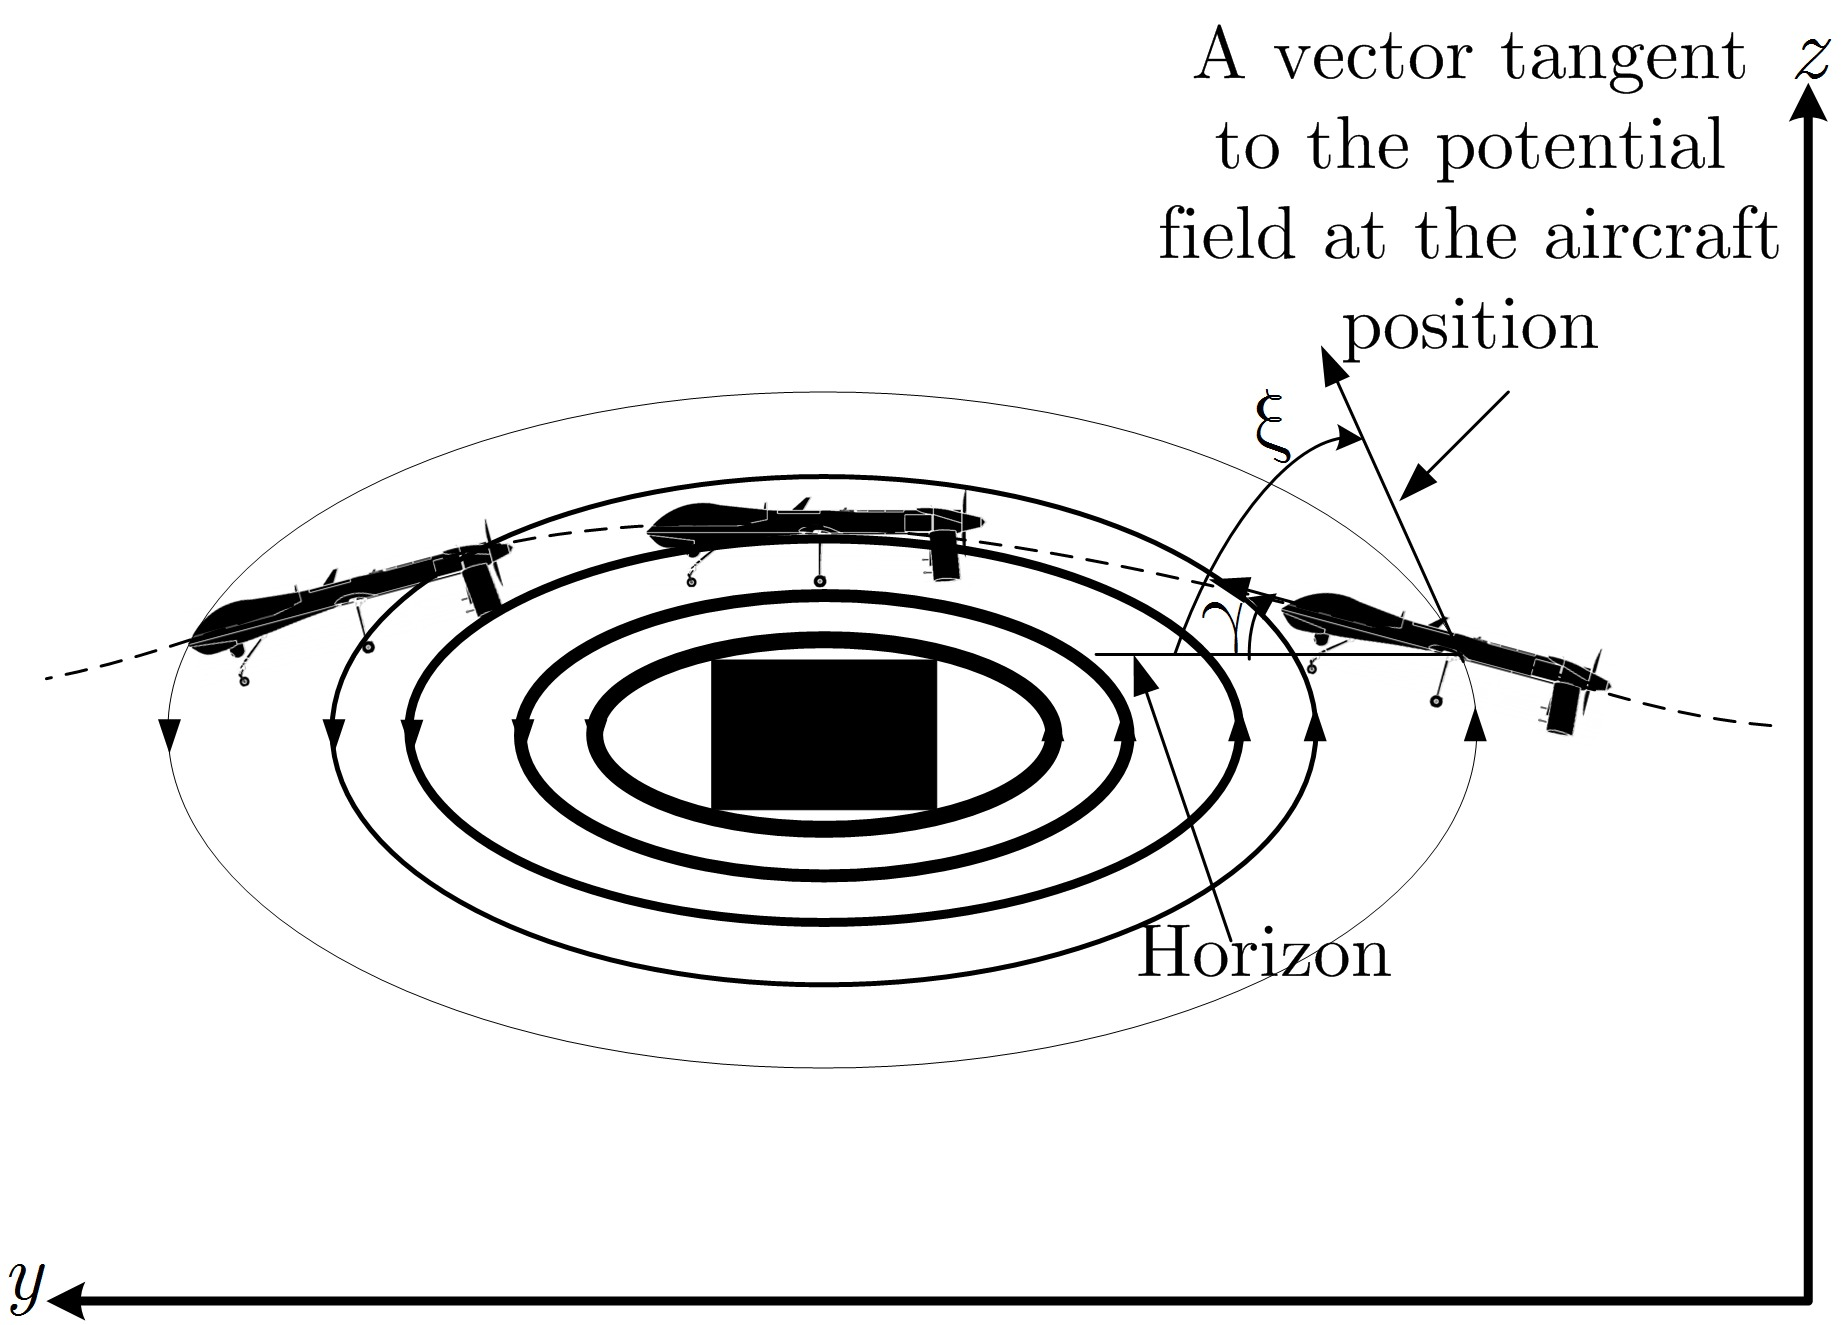
\includegraphics[width=.45\textwidth]{adap-pf_2} }
\subfigure[نمایش عملکرد \مق{APF} از بعد $y-x$]{ 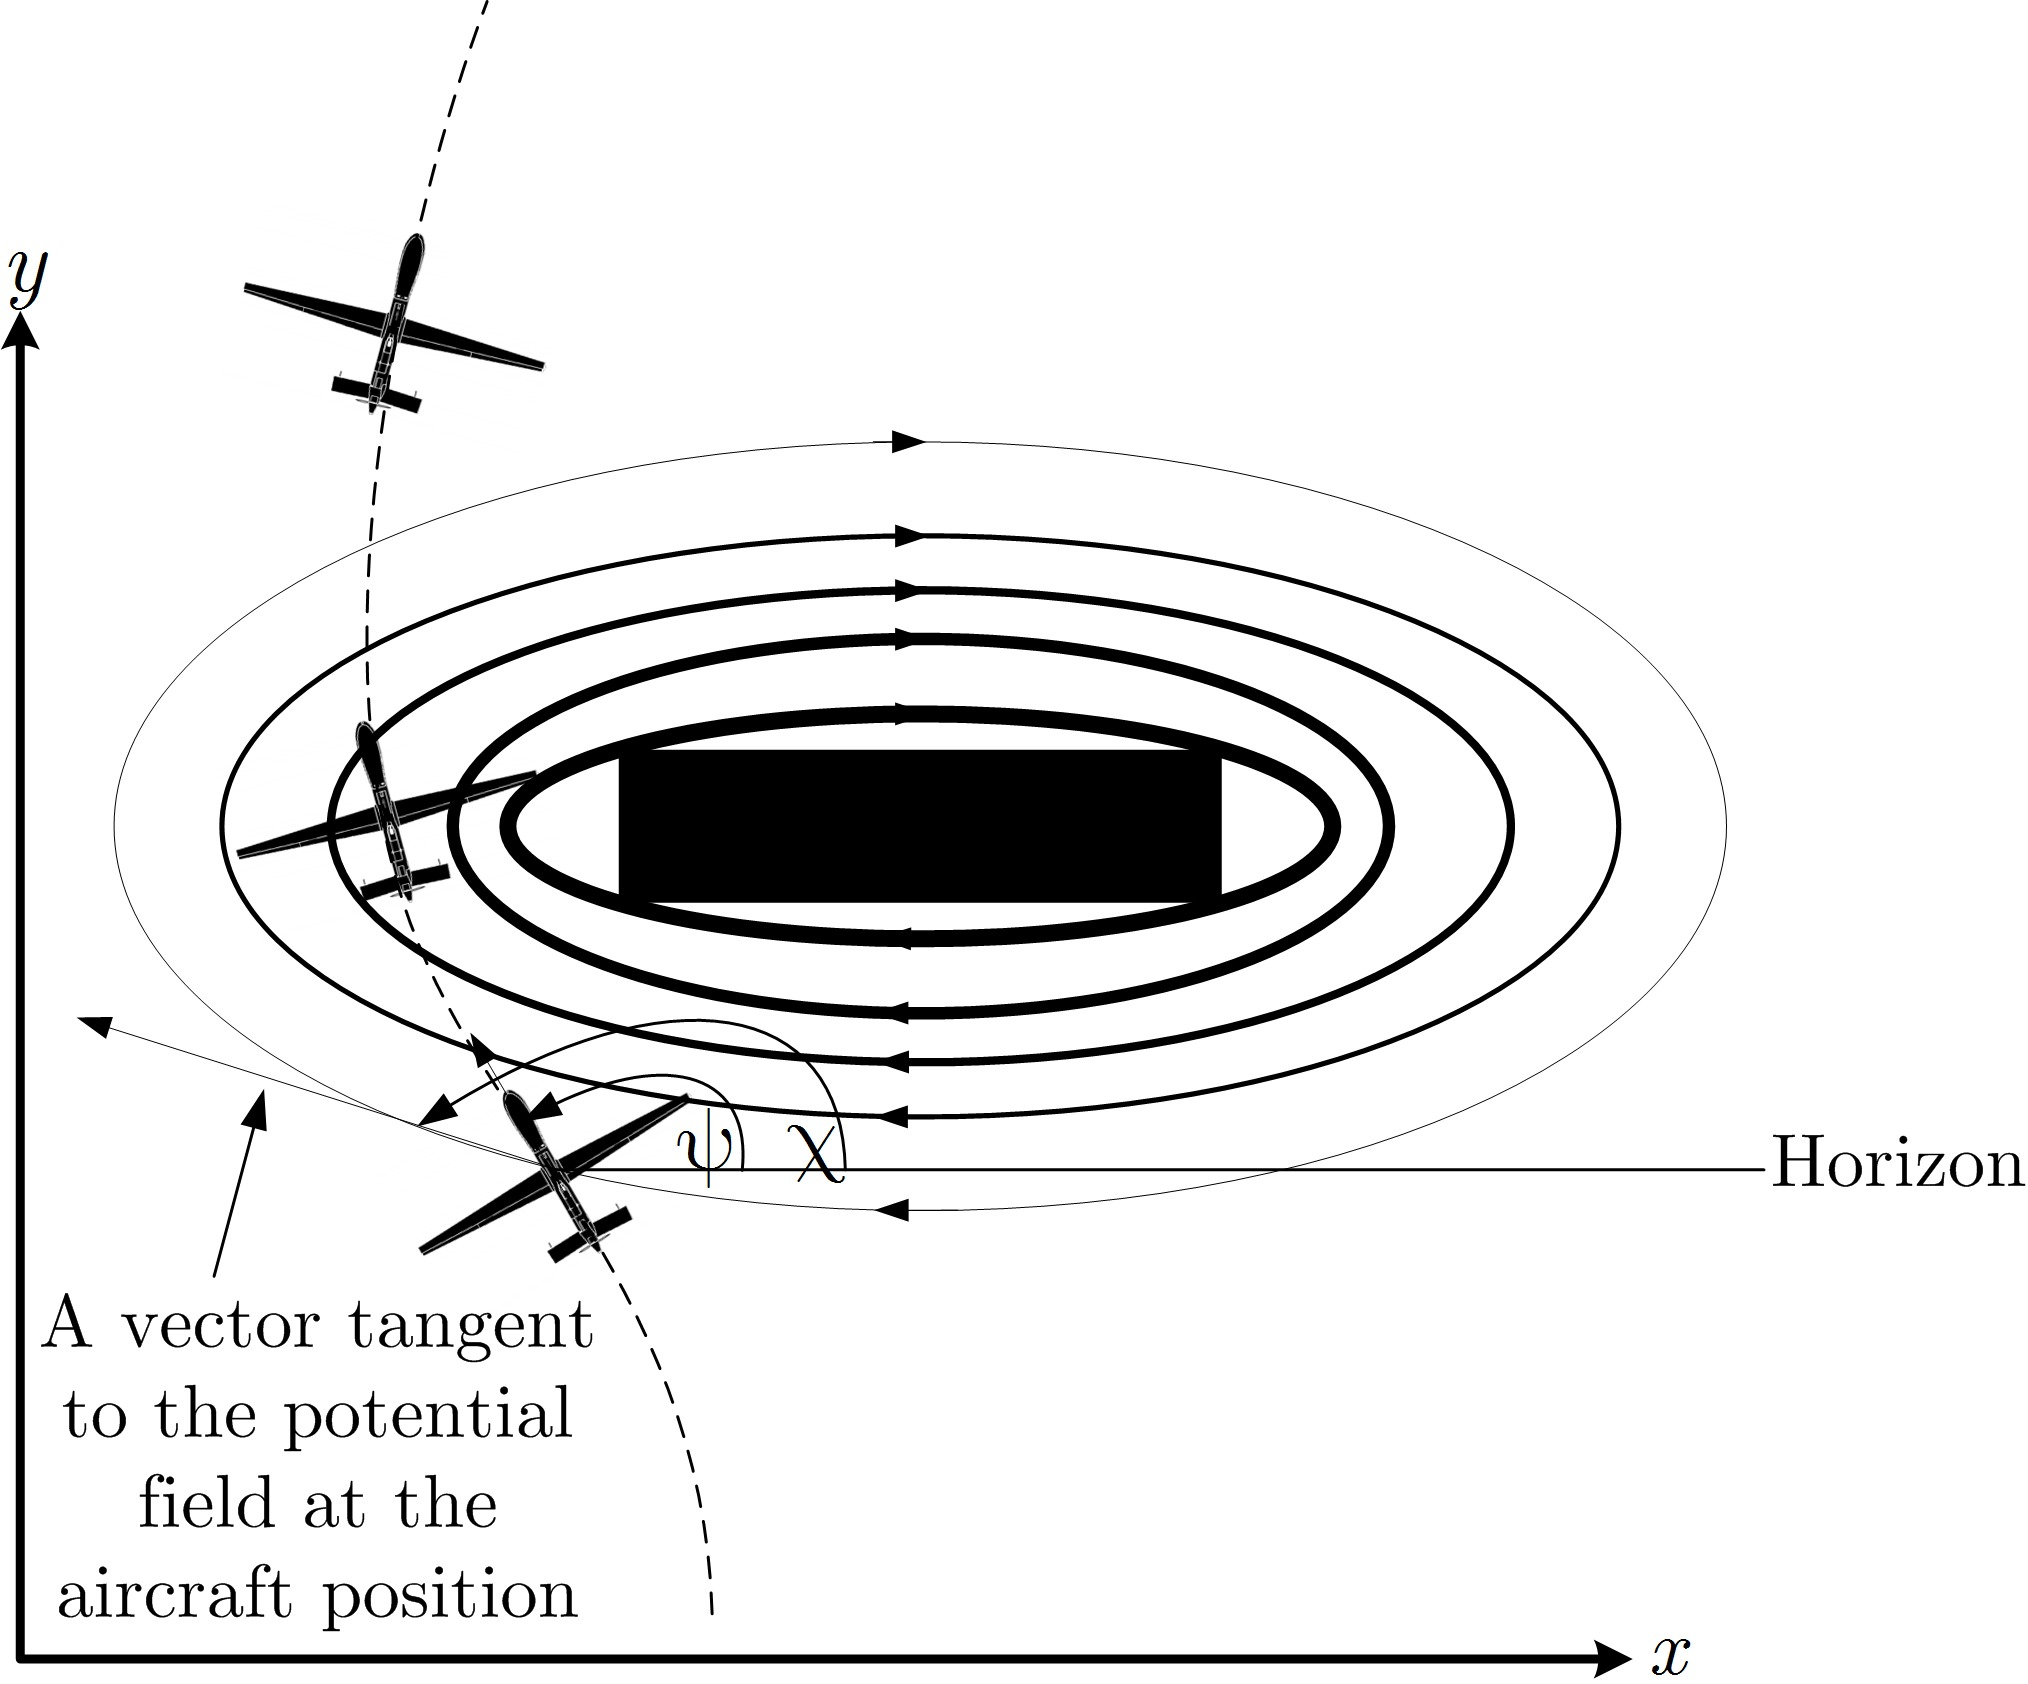
\includegraphics[width=.45\textwidth]{adap-pf_1} }
\caption{الگوریتم \مق{APF} با معرفی میدان پتانسیل چرخشی برای رفع مشکل کمینه‌ی محلی موجود در الگوریتم \مق{PF} ارائه شد.}
\label{fig:apf}
\end{figure}